\documentclass[11pt,letterpaper]{article}
\usepackage[margin=0.82in,headheight=15pt]{geometry}
\usepackage[T1]{fontenc}
\usepackage{lmodern,microtype,amsmath,amssymb,amsthm,booktabs,array,longtable,graphicx}
\usepackage{xcolor,fancyhdr,enumitem,hyperref}
\definecolor{navy}{HTML}{183447}
\definecolor{teal}{HTML}{156B73}
\hypersetup{colorlinks=true,linkcolor=teal,urlcolor=teal,citecolor=teal,pdftitle={Operational Identification of Records, Controls, and Continuous-Time Dynamics},pdfauthor={Kirtus Justus}}
\pagestyle{fancy}\fancyhf{}
\fancyhead[L]{\small\color{navy}Operational identification of records and dynamics}
\fancyhead[R]{\small Kirtus Justus}

\fancyfoot[R]{\thepage}
\setlength{\parindent}{0pt}\setlength{\parskip}{6pt}
\setlist{nosep,leftmargin=1.4em}
\renewcommand{\arraystretch}{1.15}
\newtheorem{theorem}{Theorem}[section]
\newtheorem{proposition}[theorem]{Proposition}
\newcommand{\one}{\mathbf1}
\newcommand{\TV}{\operatorname{TV}}
\newcommand{\Tr}{\operatorname{Tr}}
\newcommand{\spec}{\operatorname{spec}}
\newcommand{\rank}{\operatorname{rank}}
\newcommand{\ip}[2]{\langle #1\mid #2\rangle}
\newcommand{\ket}[1]{\lvert #1\rangle}
\newcommand{\bra}[1]{\langle #1\rvert}



\title{\color{navy}Operational Identification of Records, Controls,\\
and Continuous-Time Dynamics}
\author{Kirtus Justus}
\date{10 November 2026}
\begin{document}
\maketitle
\begin{abstract}
Identification depends on the observation and intervention class, including its
calibration parameters. We give exact ambiguity witnesses and constructive
identification results for finite-dimensional record, control and timing models.
A classical stochastic process reproduces a specified binary interference curve,
and a common environmental unitary preserves the complete reduced-system channel
while changing the product structure of environmental records. Two exact controls
identify a strictly positive, linearly minimal, stationary two-state
transition-emitting model precisely when a stated determinant is nonzero;
an explicit inverse uses short population records. Calibration uncertainty
restores an interval of compatible labelled parameters. Two positive
continuous-time Markov generators with different circulation have the same
integer-time laws, including the stated integer-boundary intervention experiments.
Two exact incommensurate intervals restore generator uniqueness, although
unbounded rates prevent uniform stable inversion. Structural propositions
separately characterize relational operations, operational composition and
invisible state extensions. Each conclusion uses an explicit mathematical model
and observation contract.
\end{abstract}

\section{Observational equivalence and identification}

Let \(\Theta\) include a model together with all admissible preparation, apparatus
and calibration parameters. For an experiment menu \(\mathcal E\), define
\[
 \theta\sim_{\mathcal E}\theta'
 \quad\Longleftrightarrow\quad
 P_\theta^e=P_{\theta'}^e
 \quad\text{for every }e\in\mathcal E.
\]
A target \(h\) is identified precisely when it is constant on every such
equivalence class. With uncertain observations and calibration, its identified
set is the range of \(h\) over the jointly compatible descriptions. This
formulation includes the nuisance parameters and distinguishes numerical
representation coordinates from invariant properties \cite{internalcollection}.

A state space, stochastic kernel or completely positive map can be used as a
formal representation. A physical interpretation adds claims about which
preparations, transformations, measurements and compositions it describes.
The results below concern the map from a declared model class to its observable
laws. Physical applicability depends on the associated access, interpretation
and calibration assumptions.

The examples address converse questions about interference curves, record
independence, hidden coordinates and sampled dynamics. A counterexample to a
converse does not invalidate its corresponding forward calculation under the
stated premises. Positive results therefore accompany the ambiguity witnesses:
added fragment access, two anchored controls and additional exact timing
information distinguish models under specified conditions.


\section{Classical realizations of a final interference curve}

A balanced two-level quantum trial with a phase setting and final binary Born readout gives, for a real record overlap $0\le\gamma\le1$,
\begin{equation}
 P(0\mid N,\phi)=\frac{1+\gamma^N\cos\phi}{2},\qquad
 N=0,1,\ldots . \label{eq:visibility}
\end{equation}
The forward derivation assumes conditionally identical product records \cite{internalcandidate}. The following construction limits what these particular recorded probabilities identify.

\begin{proposition}[Restricted classical stochastic realization]
For every allowed $\gamma$, a classical two-state process reproduces \eqref{eq:visibility} for every $N$ and every real setting $\phi$.
\end{proposition}
\begin{proof}
Let $z\in\{+1,-1\}$ start at $+1$. At each step flip its sign with probability $(1-\gamma)/2$. The transition matrix is
\[
 K_\gamma=\frac12\begin{pmatrix}1+\gamma&1-\gamma\\1-\gamma&1+\gamma\end{pmatrix}.
\]
Then $\mathbb E[z_N]=\gamma^N$. Choose the explicitly setting-dependent stochastic response
\[
 P(0\mid z,\phi)=\frac{1+z\cos\phi}{2}.
\]
All entries lie in $[0,1]$. Averaging over the hidden sign gives \eqref{eq:visibility}. Equivalently,
\[
 (1,0)K_\gamma^N
 \begin{pmatrix}(1+\cos\phi)/2\\(1-\cos\phi)/2\end{pmatrix}
 =\frac{1+\gamma^N\cos\phi}{2}.
\]
\end{proof}


\subsection{Complex overlap and a circle-valued realization}

For \(\gamma=r e^{i\delta}\), \(0\le r\le1\), the same product-record
calculation gives
\begin{equation}
 P(0\mid N,\phi)=\frac{1+\operatorname{Re}(e^{i\phi}\gamma^N)}2.
 \label{eq:complex-visibility}
\end{equation}
The visibility is \(r^N\); the argument of \(\gamma^N\) also shifts the
phase of the curve. When \(r=0\), choose \(\delta\) arbitrarily.
At \(N=0\), the empty record product has overlap one.

\begin{proposition}[Circle-valued classical realization]
The complex-overlap law has a classical circle-valued stochastic
realization for every \(|\gamma|\le1\).
\end{proposition}
\begin{proof}
Set \(\theta_0=0\) and, modulo \(2\pi\), let
\[
 \theta_{n+1}=\theta_n+\delta+\pi B_n,\qquad
 B_n\ \text{independent},\qquad P(B_n=1)=\frac{1-r}{2}.
\]
Each increment satisfies
\[
 \mathbb E[e^{i(\delta+\pi B_n)}]
 =e^{i\delta}\left(\frac{1+r}{2}-\frac{1-r}{2}\right)=\gamma.
\]
Independence gives \(\mathbb E[e^{i\theta_N}]=\gamma^N\).
Use the stochastic response
\[
 P(0\mid\theta,\phi)=\frac{1+\cos(\phi+\theta)}2.
\]
It is a probability for every \(\theta,\phi\), and its expectation is exactly
the displayed complex-overlap probability.
\end{proof}

When \(\delta=0\), the phase lies in \(\{0,\pi\}\), recovering the sign process.
For arbitrary \(\delta\), this is a circle-valued construction; it is not
being asserted to be a time-homogeneous two-state realization.

\subsection{Scope of the observational equivalence} The chosen initial preparation, $N$ noise or record steps, a phase setting, and one final binary outcome do not identify a quantum-record mechanism within a class admitting this stochastic response. Any inference from those laws alone to that mechanism fails by an exact witness.

The quantum calculation remains valid under its inputs. The construction is not a simulation of every preparation, intermediate measurement, joint effect, tensor composition, or Bell experiment. It does not establish a classical account of quantum theory. It also does not contradict a comparison against a more restricted ordinary route mixture with a fixed response: the stochastic rival here has a declared setting-dependent response. Its response calibration is an explicit part of the comparison class.

Classical-noise realizations of one-qubit dephasing have established prior art \cite{crow}. That literature often represents classical noise acting on a quantum system. The elementary construction above makes the narrower point that the specified final binary data themselves admit a fully stochastic realization. These are related claims with different scopes.

\section{System-only observations and environmental record structure}

The ambiguity persists even when both descriptions use the same quantum formalism. Hold the physical interpretation of the environmental fragment partition fixed. For the following environmental construction, take real $0\le\gamma\le1$. Put $s=\sqrt{1-\gamma^2}$ and
\[
 \ket{E_0^{(N)}}=\ket0^{\otimes N},\qquad
 \ket{E_1^{(N)}}=(\gamma\ket0+s\ket1)^{\otimes N}.
\]
The overlap is $\gamma^N$. For $N\ge2$, apply the same controlled-$Z$ unitary to fragments 1 and 2 in both branches and leave later fragments untouched:
\[
 \ket{F_j^{(N)}}=U_N\ket{E_j^{(N)}},\qquad
 U_N=\operatorname{CZ}_{12}\otimes I_{3\ldots N}.
\]
Take $U_0,U_1$ to be identities. This can be implemented as one fixed mathematical preparation rule: apply the gate after fragment 2 is created, then append later fragments normally.

\begin{proposition}[Record-independence nonidentification]
The two constructions have the same system-only channel for every system input. For $N\geq2$, the second branch of the transformed construction is entangled across fragments 1 and 2 whenever $0<\gamma<1$.
\end{proposition}
\begin{proof}
A common unitary preserves the branch overlap:
\[
 \ip{F_0^{(N)}}{F_1^{(N)}}=\ip{E_0^{(N)}}{E_1^{(N)}}=\gamma^N.
\]
At $N=2$, the transformed branch-1 coefficient matrix is
\[
 M=\begin{pmatrix}\gamma^2&\gamma s\\\gamma s&-s^2\end{pmatrix},
 \qquad\det M=-2\gamma^2s^2\ne0.
\]
A pure two-qubit vector is a product precisely when this coefficient matrix has rank one. The nonzero determinant therefore establishes entanglement. Appending product fragments preserves that distinction. For every joint input state,
\[
 \Tr_E\!\left[(I\otimes U_N)\rho_{SE}(I\otimes U_N^\dagger)\right]
 =\Tr_E\rho_{SE}.
\]
Thus the full reduced-system channel, including its action with an ancilla, is unchanged.
\end{proof}

Complete final system tomography cannot recover the specified internal environmental independence. The same conclusion applies to system-only intervention histories if the transformed fragments remain inaccessible and never recouple: the environmental unitary commutes with all later operations on the retained system and fresh fragments and disappears under the final trace. Access to old fragments, recoupling, or extra joint outcomes changes the observation menu and is outside that equivalence claim.

Consequently, $V_N=V_1^N$ is a consequence of the proposed independent-record construction, but is not sufficient evidence for its conditional independence. The conditional forward implication survives; its converse fails in the stated class.

\subsection{A large exact contrast with added environmental access}

Set $\gamma=3/5$, $s=4/5$. In the order $\ket{00},\ket{01},\ket{10},\ket{11}$,
\[
 \ket{E_1}=\frac1{25}(9,12,12,16)^T,\qquad
 \ket{F_1}=\frac1{25}(9,12,12,-16)^T.
\]
Both are normalized, and both overlap with $\ket{00}$ by $9/25$. Their coefficient determinants are $0$ and $-288/625$. The expectations of a local \(X\) observable on fragment 1 are
\[
 \langle X\otimes I\rangle_E=2\gamma s,\qquad
 \langle X\otimes I\rangle_F=2\gamma s(\gamma^2-s^2).
\]
An independently anchored branch-1 preparation and a calibrated local \(X\)
readout consequently yield
\[
 P_E(X+)=\frac{49}{50},\qquad P_F(X+)=\frac{457}{1250},
 \qquad P_E(X+)-P_F(X+)=\frac{384}{625}=0.6144.
\]
This separates the displayed pair. It does not identify all possible environmental mechanisms. The distinction also depends on a fixed, accessible fragment partition: if arbitrary entangling changes of factorization are declared a gauge, the purported independence property changes its meaning. The branch preparation, fragment access and readout are additional
assumptions. If each reported binary law can move by TV at most \(\varepsilon\),
the remaining interval gap is at least \(384/625-2\varepsilon\); positivity of
this quantity is sufficient for uniform pair separation.



\section{Identification by two exact controls}

Consider a row-convention, binary-output transition-emitting model with positive matrices $T_0,T_1$, stochastic sum, and an unanchored stationary preparation $\pi$. Assume its passive process is linearly minimal of dimension two:
the linear representation is reachable and observable. For a word
\(w=y_1\cdots y_m\), its probability is
\(P(w)=\pi T_{y_1}\cdots T_{y_m}\one\). Each experiment starts from the
model's stationary preparation. Positive hidden-state similarity equivalence is established realization theory; its model-class conditions matter \cite{vanluyten}.

Consider the example \cite{internalintervention}
\[
 T_0=\frac1{20}\begin{pmatrix}6&2\\1&3\end{pmatrix},\quad
 T_1=\frac1{20}\begin{pmatrix}4&8\\7&9\end{pmatrix},\quad
 \pi=(4/9,5/9).
\]
Its two-output probability matrix has determinant $53/8100$, so its linear dimension is two. One fixed silent control does not identify this unrestricted positive class: a small similarity commuting with that control preserves every permitted controlled word law. Strict positivity supplies an admissible neighborhood. Linear minimality prevents a nonidentity similarity from fixing the whole realization.

Now anchor two controls in the same consistently labelled hidden coordinate basis:
\[
 K_j=\begin{pmatrix}1-a_j&a_j\\b_j&1-b_j\end{pmatrix},
 \qquad 0\le a_j,b_j\le1,\qquad \Delta=a_1b_2-a_2b_1.
\]
The controls are held fixed across candidates, not transformed along with them.

\begin{theorem}[Exact two-control criterion]
Within the stated strictly positive, stationary, linearly minimal two-state class, the controlled laws identify the numerical preparation and output matrices if and only if $\Delta\ne0$. When identification holds, records with at most one control followed by at most two output symbols suffice at the population-probability level.
\end{theorem}

\begin{proof}
Write $\pi=(r,1-r)$, $e=T_0\one=(e_1,e_2)^T$, $d=e_1-e_2$, and $k=rd$. If $d=0$, both output matrices send $\one$ to scalar multiples of $\one$, and all passive words have an iid rank-one law. Hence $d\ne0$ in the stated class.

Observe $q=P(0)$ and $q_j=P(K_j\text{ then }0)$. Direct multiplication gives
\begin{equation}
 \begin{pmatrix}q_1-q\\q_2-q\end{pmatrix}
 =B\begin{pmatrix}d\\k\end{pmatrix},\qquad
 B=\begin{pmatrix}b_1&-(a_1+b_1)\\b_2&-(a_2+b_2)\end{pmatrix},
 \quad \det B=\Delta. \label{eq:B}
\end{equation}
For $\Delta\ne0$, recover
\[
 d=\frac{-(a_2+b_2)(q_1-q)+(a_1+b_1)(q_2-q)}{\Delta},\qquad
 k=\frac{-b_2(q_1-q)+b_1(q_2-q)}{\Delta},
\]
and then $r=k/d$, $e_2=q-k$, $e_1=q-k+d$. At least one $q_j-q$ is nonzero because $B$ is invertible and $d\ne0$. For that $j$, set
\[
 A=\begin{pmatrix}\pi\\\pi K_j\end{pmatrix},\qquad
 F=\begin{pmatrix}1&e_1\\1&e_2\end{pmatrix},\qquad
 C_y=\begin{pmatrix}P(y)&P(y0)\\P(K_j\text{ then }y)&P(K_j\text{ then }y0)\end{pmatrix}.
\]
The observed matrices satisfy $C_y=AT_yF$. Since
\[
 \det A=-\frac{q_j-q}{d},\qquad\det F=-d,
\]
both inverses exist, giving $T_y=A^{-1}C_yF^{-1}$.

For necessity, every row-sum-zero $2\times2$ perturbation has form
\[
 X=\begin{pmatrix}-x&x\\y&-y\end{pmatrix}.
\]
Commutation with $K(a,b)$ is equivalent to $bx-ay=0$. If $\Delta=0$, the two controls commute and share a nonzero admissible infinitesimal similarity direction. Choose a nonidentity control $K$ and $S_t=I+t(K-I)$; if both controls are identities, choose any nontrivial small row-stochastic similarity instead. Small $t$ preserves positivity, normalization, and stationarity under
\[
 T_y\mapsto S_t^{-1}T_yS_t,\qquad\pi\mapsto\pi S_t.
\]
The fixed controls commute with $S_t$, so every controlled law telescopes to the original law. A linearly reachable minimal realization cannot be fixed by a nonidentity $S_t$: such a matrix would fix every reachable row. The resulting continuum is not exhausted by the two label permutations.
\end{proof}

\subsection{Exact reconstruction with positive non-reset controls}

Take
\[
 K_1=\begin{pmatrix}3/4&1/4\\1/2&1/2\end{pmatrix},\qquad
 K_2=\begin{pmatrix}1/2&1/2\\1/4&3/4\end{pmatrix},\qquad\Delta=-3/16.
\]
Neither is a reset or permutation. The example yields
\[
 q=\frac{13}{45},\quad q_1=\frac{29}{90},\quad q_2=\frac{49}{180},
 \qquad d=\frac15,\quad k=\frac4{45}.
\]
For $j=1$,
\[
 C_0=\begin{pmatrix}13/45&9/100\\29/90&21/200\end{pmatrix},\qquad
 C_1=\begin{pmatrix}32/45&179/900\\61/90&337/1800\end{pmatrix}.
\]
The reconstruction returns exactly the stated $\pi,T_0,T_1$. Replacing $K_2$ by $K(1/8,1/4)$ gives an adverse control with $\Delta=0$ and preserves the original ambiguity.

This is an exact identification statement within the stated class. The short record length is not a number of experimental trials or a finite-sample stability guarantee. Conditioning worsens as $|\Delta|$, $|d|$, or the selected displacement $|q_j-q|$ becomes small. Naming a control matrix does not establish its physical calibration.



\section{Calibration uncertainty and an identified-set interval}

For the same example and controls, put
\[
 S_t=\begin{pmatrix}1-t&t\\2t&1-2t\end{pmatrix},\qquad 0\le t\le\frac1{10}.
\]
Direct multiplication gives
\begin{align*}
 S_t^{-1}K_1S_t&=K_1,\\
 S_t^{-1}K_2S_t-K_2&=
 \begin{pmatrix}3t/4&-3t/4\\3t/4&-3t/4\end{pmatrix},\\
 \pi_t=\pi S_t&=((4+6t)/9,(5-6t)/9).
\end{align*}
The transformed output matrices are
\[
 T_{0,t}=\frac1{20(1-3t)}
 \begin{pmatrix}
 6-15t-t^2&2-5t+t^2\\
 1-8t-t^2&3-12t+t^2
 \end{pmatrix},
\]
\[
 T_{1,t}=\frac1{20(1-3t)}
 \begin{pmatrix}
 4-3t-35t^2&8-37t+35t^2\\
 7-4t-35t^2&9-36t+35t^2
 \end{pmatrix}.
\]
On the stated interval, entrywise lower bounds for their numerator matrices are
\[
 \begin{pmatrix}449/100&3/2\\19/100&9/5\end{pmatrix},\qquad
 \begin{pmatrix}67/20&43/10\\25/4&27/5\end{pmatrix}.
\]
Since \(1-3t\ge7/10\), the outputs remain strictly positive. The transformed
preparation and controls are positive and normalized as well. The second control's maximum row total-variation change is $3t/4$; the first remains exactly fixed. Simultaneously transforming the model, preparation, and second control preserves every controlled output law by telescoping.

\begin{proposition}[A constructive width bound]
Suppose $K_1$ is exact and the admissible $K_2$ calibration class contains all row-stochastic matrices within maximum row-TV distance $\varepsilon\ge0$ of its nominal value. With no separate anchor on $\pi$ and no additional calibration observations that exclude the displayed family, the projection of the compatible set onto its labelled first preparation mass contains
\begin{equation}
 \left[\frac49,\ \frac49+\min\left\{\frac1{15},\frac{8\varepsilon}{9}\right\}\right].
 \label{eq:width}
\end{equation}
\end{proposition}
\begin{proof}
Every $t\in[0,\min\{1/10,4\varepsilon/3\}]$ is admissible, gives the same controlled law, and has first mass $4/9+2t/3$. Taking its range proves the claim.
\end{proof}

At $\varepsilon=1/100$, choose $t=1/75$. The second control changes by exactly $1/100$ in each row-TV distance, while a certified compatible subinterval is
\[
 [4/9,34/75],\qquad\text{width}=2/225=0.008888\ldots .
\]
Thus the width is at least $0.8888\ldots$ percentage points, even with exact knowledge of all permitted output probabilities. This is a constructive lower bound, not a global sharp characterization. The target is a labelled latent coordinate, not a similarity-invariant physical property. If one identifies gauge-related numerical descriptions as the same model, the target must be reformulated accordingly.

More generally, consider a linearly minimal model of dimension \(n\ge2\)
with positive output matrices and a positive unanchored preparation. Suppose a
finite menu of strictly positive controls has calibration classes containing
relative open neighborhoods within the row-stochastic matrices, and the
admissible model class allows the corresponding local changes. Choose a
nonidentity invertible row-stochastic \(S\) sufficiently near \(I\), transform
all outputs and controls by \(M\mapsto S^{-1}MS\), and transform
\(\pi\mapsto\pi S\). Positivity and neighborhood membership survive by
continuity. The finite number of controls permits one common sufficiently small
choice. Every controlled law is preserved by telescoping, while linear
reachability prevents \(S\ne I\) from fixing the entire realization. Additional noisy controls can narrow an identified set without making every coordinate a point. Exactly known structural zeros, independently anchored preparations, or separately modelled calibration outcomes can remove this particular freedom and require their own analysis.


\subsection{Pair discrimination under reset error}

Pair discrimination and identification of a whole class have different
quantifiers. For the displayed output matrices, use
\[
 S=\begin{pmatrix}9/10&1/10\\1/5&4/5\end{pmatrix},\qquad
 T_y'=S^{-1}T_yS,\qquad\pi'=\pi S.
\]
This pair has the same passive law. Under an exactly common \(K(a,b)\), its
one-output contrast is \((2a-b)/35\). If \(b=2a\), the control commutes with
\(S\) and all controlled laws agree. Otherwise the one-output contrast
already separates the pair.

A nominal reset to state 2 with wrong-state mass \(u\in[0,\delta]\) gives
output-zero probability \((1+u)/5\) in the first model and \((1+2u)/7\)
in the second. Allowing the nuisance to differ between candidates, the
probability intervals are
\[
 [1/5,(1+\delta)/5],\qquad [1/7,(1+2\delta)/7].
\]
They are disjoint precisely when \(\delta<1/5\).
At \(\delta=1/5\), the first model's exact reset \(R_2=\one(0,1)\) and
the second model's admissible reset
\[
 S^{-1}R_2S=\one(1/5,4/5)
\]
give the same laws for every word formed from outputs and this reset.
The same holds for common adaptive visible-history policies. This proves
sharpness of the threshold for this pair and this nuisance class.
Additional per-output TV error \(\varepsilon\) leaves the sufficient
positive-gap condition \(2/35-2\delta/7-2\varepsilon>0\).

For ideal iid reset trials of this simple pair, take the null output-zero
probability \(p_0=1/7\) and the alternative \(p_1=1/5\). The exact randomized
fixed-horizon size-\(0.05\) test first attains power at least \(0.95\) at
468 trials; 467 does not suffice \cite{internalintervention}. This boundary
does not optimize adaptive policies or apparatus cost, and supplies no
sample size for the new reconstruction and calibration-set problems.


\section{Sampled transitions and continuous-time circulation}

Consider a labelled three-state space, homogeneous continuous-time Markov dynamics and an exact reference sampling interval. These define the model class and timing contract. The question is whether the sampled transition law identifies the generator. Time below is measured in units of the reference interval.

Let
\[
 C=\begin{pmatrix}0&1&0\\0&0&1\\1&0&0\end{pmatrix},\quad
 \Pi=\frac13\one\one^T,\quad R=I-\Pi,\quad A=C-C^2.
\]
Define
\begin{equation}
 Q_0=-12R=4(C+C^2-2I),\qquad
 Q_1=Q_0+\frac{2\pi}{\sqrt3}A. \label{eq:generators}
\end{equation}
Both have zero row sums and strictly positive off-diagonal entries: the latter rates are $4\pm2\pi/\sqrt3$. Both have the uniform stationary distribution.

\begin{theorem}[A positive three-state sampled-law ambiguity]
The generators in \eqref{eq:generators} obey $e^{nQ_0}=e^{nQ_1}$ for every nonnegative integer $n$. They are not similar and are not related by a positive scalar time rescaling. The first satisfies detailed balance with its stationary distribution; the second does not.
\end{theorem}
\begin{proof}
The identities $A\Pi=\Pi A=0$, $A^2=-3R$, and $Q_0A=AQ_0$ yield
\begin{align}
 e^{tQ_0}&=\Pi+e^{-12t}R,\\
 e^{tQ_1}&=\Pi+e^{-12t}\left[\cos(2\pi t)R+
 \frac{\sin(2\pi t)}{\sqrt3}A\right]. \label{eq:semigroup}
\end{align}
At every integer $t=n$ the bracket equals $R$. Their spectra are
\[
 \spec(Q_0)=\{0,-12,-12\},\qquad
 \spec(Q_1)=\{0,-12+2\pi i,-12-2\pi i\}.
\]
These exclude similarity and scalar time rescaling. $Q_0$ is symmetric; $Q_1$ is not. For $Q_1$, the uniform stationary edge current is
\[
 \frac13\bigl((Q_1)_{12}-(Q_1)_{21}\bigr)=\frac{4\pi}{3\sqrt3}>0.
\]
\end{proof}

This is an explicit instance of the established Markov embedding ambiguity and system aliasing \cite{baake,yue}. In particular, sampled reversibility need not imply generator reversibility.

\subsection{Which experiments remain equivalent?}

The initial distribution may be any common labelled preparation, not just the stationary one. If every intervention and readout occurs at integer boundaries, so every uncontrolled interval has a nonnegative integer duration, the conditional transition matrices are the same. Any sequence of common instantaneous stochastic state maps and boundary instruments therefore has the same outcome law. Adaptive choices and scheduling on this same integer grid also give equality: by induction, each common observed history has the same next-action rule and conditional outcome distribution.

This does not cover controls that modify the subsequent generator, continuous monitoring, jump counts, waiting-time observations, or intermediate readouts. Those supply additional information. The equality also presupposes that all unrecorded evolution between interventions is generated by the fixed $Q_0$ or $Q_1$.

\subsection{A positive intermediate-time control}

At one quarter of the reference interval, \eqref{eq:semigroup} gives
\[
 (e^{Q_1/4})_{12}-(e^{Q_1/4})_{13}
 =\frac{2e^{-3}}{\sqrt3}=0.0574891546486971\ldots,
\]
whereas the same oriented contrast is zero for $Q_0$. A calibrated preparation of state 1 and a readout resolving states 2 and 3 therefore distinguish the pair at this interval. This is a contrast between two outcome probabilities, not an optimized statistical power claim.

\begin{center}
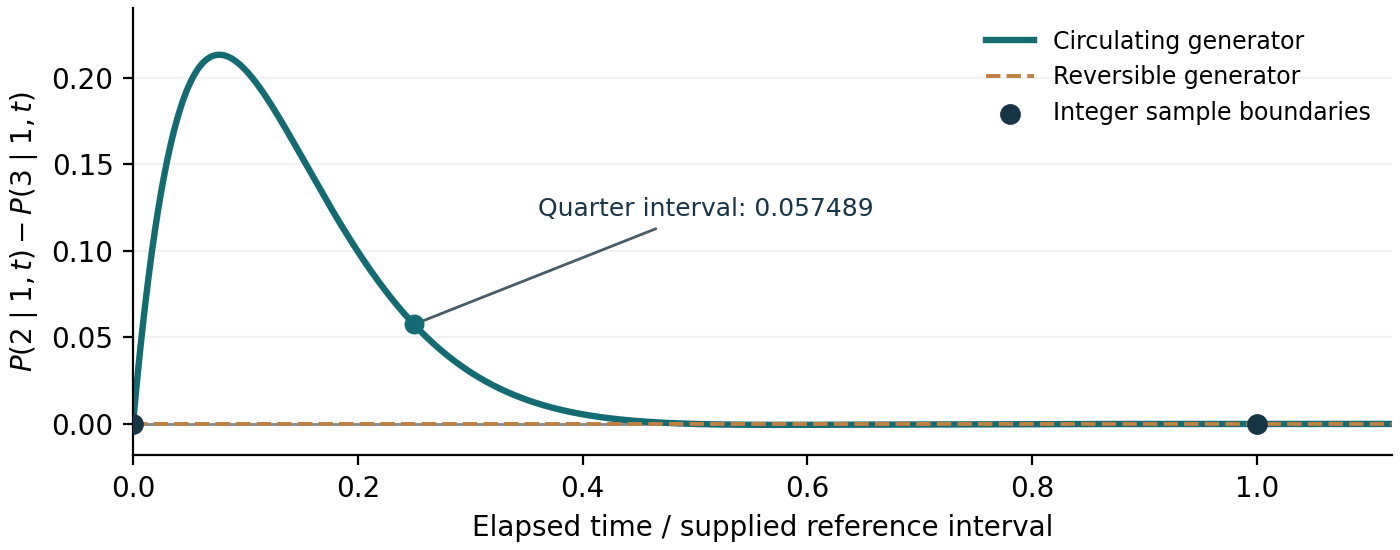
\includegraphics[width=0.88\textwidth]{Temporal_Contrast.png}
\end{center}
{\small\textbf{Figure 1.} Analytic oriented contrast from the two generators. Integer-boundary observations see the same transition matrix. The displayed intermediate contrast requires additional timing and labelled-state access. The plotted parameter is a ratio to the reference observation interval.}



\section{Additional timing information and stable inversion}

The sampled-law obstruction does not imply that continuous generators are never identifiable.

\begin{theorem}[Two exact incommensurate intervals]
Let $Q,B$ be finite square matrices in the same labelled coordinate basis. Suppose $t_1,t_2>0$, $t_1/t_2$ is irrational, and
\[
 e^{t_1Q}=e^{t_1B},\qquad e^{t_2Q}=e^{t_2B}.
\]
Then $Q=B$.
\end{theorem}
\begin{proof}
Denote the common exponentials by $M_1,M_2$. They commute and are invertible. For every pair of integers $m,n$,
\[
 e^{(mt_1+nt_2)Q}=M_1^mM_2^n=e^{(mt_1+nt_2)B}.
\]
The additive subgroup $\{mt_1+nt_2:m,n\in\mathbb Z\}$ is dense in $\mathbb R$. Continuity gives equality of the two matrix exponentials for all real times. Differentiation at zero gives $Q=B$. Negative powers are only an algebraic step; no physical negative-time operation is assumed.
\end{proof}

The theorem requires exact full transition matrices, a common finite-dimensional time-homogeneous model, consistently labelled states, and known intervals with the stated ratio. A finite measurement cannot certify an irrational real number by decimal precision alone. This result describes population-level identification under a mathematical timing contract. It does not give an automatic experimental certification method or a physical clock.

\subsection{Exact uniqueness is not uniform stability}

Fix $c\ne0$ and use the same $R,A$ as above. For $a>3|c|$, both
\[
 Q_a=-aR,\qquad B_a=-aR+cA
\]
are Markov generators with strictly positive off-diagonal rates. Their matrix difference $cA$ is fixed and nonzero. Yet
\[
 e^{tB_a}-e^{tQ_a}
 =e^{-at}\left[(\cos(\sqrt3ct)-1)R+
 \frac{\sin(\sqrt3ct)}{\sqrt3}A\right]
\]
tends to zero at every fixed positive observation time as $a\to\infty$. It also tends uniformly to zero over any fixed finite list of positive intervals. Thus arbitrarily precise-looking transition matrices need not give a uniformly small generator error over an unbounded rate class, even when exact two-interval uniqueness applies.

A specified compact generator class restores qualitative uniform inverse continuity: otherwise pairs with observational distance tending to zero and generator distance bounded below would have a convergent subsequence contradicting exact injectivity. This is the standard compactness mechanism for the inverse of a continuous injective observation map \cite{internalcollection}. It supplies no numerical rate by itself. A useful finite-data design still needs rate bounds, timing uncertainty, measurement error, conditioning, and an acquisition contract.


\section{Structural constraints on relational and operational models}

These statements concern explicit structural assumptions. They do not select
a physical interpretation of a relational signature, observation map or
composition law.

\subsection{Initial and terminal objects}

Fix a relational signature of positive arities and the category of finite
nonempty structures with all relation-preserving homomorphisms.

\begin{proposition}
The empty-relation singleton is weakly initial, the full singleton is terminal,
and this category has no initial object.
\end{proposition}
\begin{proof}
For the empty-relation singleton \(E\), every function \(E\to A\) is a
homomorphism, so
\(|\operatorname{Hom}(E,A)|=|A|\). This is nonzero but need not be one.
For the full two-point structure \(F_2\), every function \(A\to F_2\) is a
homomorphism. Thus
\[
 |\operatorname{Hom}(A,F_2)|=2^{|A|}\ge2,
\]
which excludes any nonempty initial object.
The unique function from any \(A\) to the full singleton is a homomorphism,
proving terminality.
\end{proof}

These use the standard unique-morphism universal properties
\cite{stacksinitial}. In the thin homomorphism preorder, parallel arrows
are identified and \(E\) represents a least element. Neither the finite-core
theorem nor the operational-rank proof below requires \(E\) to be initial
in the full category.

\subsection{Inverse limits with a greatest context}

Let a context poset have greatest element \(K\), and let sets \(C(i)\)
have coherent restriction maps \(r_{ji}:C(j)\to C(i)\) for \(i\le j\).

\begin{proposition}
The inverse limit is canonically isomorphic to \(C(K)\), which need not
be a singleton.
\end{proposition}
\begin{proof}
Each \(x\in C(K)\) determines the compatible family
\((r_{Ki}(x))_i\). Conversely, every compatible family is determined by its
\(K\) coordinate. Projection to that coordinate is the inverse map.
\end{proof}

A two-point top fiber and singleton lower fibers give exactly two compatible
families. Surjectivity is not required. The argument realizes the usual
set-valued diagram-limit definition \cite{stackslimit}.

\subsection{Natural deterministic operations on equivalence relations}

Fix a finite nonnegative integer \(r\). For every finite set \(S\), let
\[
 F_S:\operatorname{Eq}(S)^r\longrightarrow\operatorname{Eq}(S)
\]
be a total deterministic operation that commutes with restriction along
every injection.

\begin{theorem}
There are exactly \(2^r+1\) such operations: intersections over selected
subsets of the inputs, including the empty intersection, and the constant
discrete relation. For \(r=2\), commutativity and pointwise idempotence
\(F_S(R,R)=R\) leave intersection alone.
\end{theorem}
\begin{proof}
Restriction to two distinct points and relabelling show that their output
bit is a single Boolean function \(f:\{0,1\}^r\to\{0,1\}\) of the input
pair bits. Put \(\mathcal F=f^{-1}(1)\).

If \(u\in\mathcal F\) and \(v\ge u\), assign the pair vectors
\((u,u,v)\) to \(12,23,13\) on three points. Each coordinate is a valid
equivalence pattern: \(000\), \(001\) or \(111\). Output transitivity gives
\(v\in\mathcal F\). Similarly, if \(u,v\in\mathcal F\), the pair vectors
\((u,v,u\wedge v)\) are valid, and transitivity gives
\(u\wedge v\in\mathcal F\).

Thus \(\mathcal F\) is upward closed and intersection closed. If nonempty,
its finite meet \(c=\bigwedge_{u\in\mathcal F}u\) belongs to \(\mathcal F\)
and \(\mathcal F=\{u:u\ge c\}\). Consequently \(f\) is conjunction over
the inputs selected by the 1-bits of \(c\).
If \(\mathcal F\) is empty, the output is the discrete relation.
Conversely, all the indicated operations preserve equivalence relations
and commute with every restriction.

There are \(2^r\) subsets and one additional discrete constant.
In the binary case the five operations are discrete, intersection, the
two projections and universal. Commutativity excludes the projections,
while pointwise idempotence excludes both constants.
\end{proof}

The theorem yields five binary and nine ternary operations. Its all-size
conclusion follows from exact naturality and the transitivity argument.

\subsection{Operational rank under idempotent composition}

Let \(r(x)\) denote the rank of the preparation-effect pairing for an
operational object \(x\). A finite rank can be witnessed by normalized
preparations and effects with a nonsingular evaluation matrix.
Assume that independent preparations and product effects are available
for \(x\wedge y\), with factorizing evaluations
\[
 (e\otimes f)(p\otimes q)=e(p)f(q).
\]
These are additional operational assumptions \cite{internalcandidate}.

\begin{proposition}
Under these assumptions, for objects of finite operational ranks \(r(x)\) and \(r(y)\),
\[
 r(x\wedge y)\ge r(x)r(y).
\]
If composition is idempotent as an operational object, so that
\(r(x\wedge x)=r(x)\), a finite positive \(r(x)\) must equal one.
\end{proposition}
\begin{proof}
Take nonsingular evaluation matrices \(A,B\) witnessing the two ranks.
The product preparations and effects give \(A\otimes B\), whose rank is
\(r(x)r(y)\). This proves the inequality.
Idempotence gives \(r(x)\ge r(x)^2\), forcing a positive finite integer
rank to be one.
\end{proof}

This requires linear separation by effects, not perfect single-shot
discrimination of every preparation. The preparation, effect and product
assumptions do not follow from a relational signature alone.

\subsection{A local associator bound for stochastic operations}

For each finite \(S\), let
\[
 \mathcal K_S:\operatorname{Eq}(S)^2
 \longrightarrow\mathcal P(\operatorname{Eq}(S))
\]
be a probability kernel with exact restriction compatibility under every
injection, symmetry in its inputs and pointwise idempotence
\(\mathcal K_S(R,R)=\delta_R\). Kernel composition uses successive
conditional sampling. On two positions, denote the discrete and universal
relations by \(0,1\). The mixed-input output is \(1\) with probability \(a\).

\begin{proposition}
These assumptions imply \(a\le1/2\). The associator at the ordered
two-position inputs \((1,1,0)\) has TV distance \(a(1-a)\).
If this discrepancy is at most \(\varepsilon_2\), then
\(a\le2\varepsilon_2\).
For general \(R,Q\), let \(\kappa\) count unordered pairs of distinct
\(R\cap Q\) blocks that are related by exactly one of \(R,Q\). Then
\[
 \TV(\mathcal K_S(R,Q),\delta_{R\cap Q})
 \le\min\{1,\kappa a\}.
\]
\end{proposition}
\begin{proof}
Use three positions with \(12\) related only in the first input, \(23\)
only in the second and \(13\) in neither. The first two output mergers
each have probability \(a\), while the third pair remains unrelated
almost surely. The first two events are disjoint by output transitivity,
so \(2a\le1\).

On inputs \((1,1,0)\), the left-associated merger probability is \(a\).
The right-associated probability is \(a+(1-a)a=2a-a^2\).
Their binary-law TV distance is \(a(1-a)\ge a/2\), proving the local bound.

For a general carrier, every pair within a common block has input bits
\((1,1)\) and stays related almost surely. A pair unrelated in both inputs
has bits \((0,0)\) and stays unrelated. Any departure from \(R\cap Q\)
therefore merges an eligible pair of distinct common blocks. Restriction
compatibility gives probability \(a\) for each such merger. The union
bound gives probability at most \(\kappa a\) for any departure.
This is the TV distance from the point mass at \(R\cap Q\).
\end{proof}

The proof needs a two-position population associator and exact structural
restrictions. It does not require a uniform all-carrier associator bound.
The result depends on size through \(\kappa\); finite observations do not
establish exact naturality at every size.

\subsection{Invisible state extensions}

Let \(K_u(x,x')\) be stochastic visible-state kernels for actions \(u\).
For arbitrary stochastic hidden-state kernels \(L_u(z,z')\), define
\[
 \widetilde K_u((x,z),(x',z'))=K_u(x,x')L_u(z,z').
\]
Choose any initial joint distribution with the prescribed visible marginal.

\begin{proposition}
Projection to \(x\) has the original visible law under every common
policy based only on visible history.
\end{proposition}
\begin{proof}
For every \(x,z,x',u\),
\[
 \sum_{z'}\widetilde K_u((x,z),(x',z'))=K_u(x,x').
\]
The next visible transition is therefore independent of the hidden state
and has the original conditional law. Induction proves the result for
deterministic or randomized visible-history policies and common readouts
depending only on the visible states.
\end{proof}

These extensions obstruct latent-state-count inference in the unrestricted
class. They are not minimal-realization counterexamples; the similarities
in Section 4 address that distinct problem. Whether an invisible extension
is additional physical structure or a redundant description requires
a separate interpretive criterion.



\section{Identified sets, stability and further mathematical questions}

The observation menu controls both negative and positive conclusions.
A final-output classical realization does not settle unrestricted quantum
experiments. System-channel equivalence need not persist with access to
environmental fragments. Exact-control reconstruction does not establish
physical calibration, and exact timing uniqueness does not supply uniform
stable inversion without quantitative restrictions.

A natural next problem is a two-sided identified-set bound under joint
control-calibration uncertainty and finite sampling. The explicit inverse
exposes dependence on \(|\Delta|\), the emission gap \(|d|\) and the
displaced preparation. The similarity family supplies an unavoidable lower
bound in one declared nuisance class. A matching upper bound must specify
the complete admissible class and distinguish invariant predictions from
coordinates that move under allowed similarities.

For environmental records, a further problem is to characterize which
factorization properties become identifiable under specified fragment
measurements and recouplings. For continuous-time dynamics, a quantitative
modulus on bounded generator classes would connect exact uniqueness with
noisy transition estimates and uncertain timing.

These are conditional mathematical questions. Physical application requires
a justified correspondence between the formal objects and admissible
preparations, transformations, retained outcomes and time measurements.
Uniqueness of a total underlying description is not required for every
useful prediction; the predicted target must instead be invariant over
the descriptions that the stated experiment cannot distinguish.



\section*{Acknowledgments}
Kirtus Justus directed the research. ChatGPT (OpenAI) assisted with the
derivations, source inspection, computational checks and preparation of this
manuscript. The unpublished manuscripts cited below belong to the same research
program and are not independent sources of empirical confirmation.

\begin{thebibliography}{99}
\bibitem{crow}
D. Crow and R. Joynt, \emph{Classical simulation of quantum dephasing and
depolarizing noise}, Physical Review A \textbf{89}, 042123 (2014).
\href{https://doi.org/10.1103/PhysRevA.89.042123}{doi:10.1103/PhysRevA.89.042123}.
\href{https://arxiv.org/abs/1309.6383}{arXiv:1309.6383}.

\bibitem{vanluyten}
B. Vanluyten, J. C. Willems, and B. De Moor,
\emph{Equivalence of state representations for hidden Markov models},
Systems \& Control Letters \textbf{57}, 410--419 (2008).
\href{https://doi.org/10.1016/j.sysconle.2007.10.004}{doi:10.1016/j.sysconle.2007.10.004}.

\bibitem{baake}
M. Baake and J. Sumner, \emph{Notes on Markov embedding},
Linear Algebra and its Applications \textbf{594}, 262--299 (2020).
\href{https://arxiv.org/abs/1903.08736}{arXiv:1903.08736}.

\bibitem{yue}
Z. Yue, J. Thunberg, and J. Goncalves,
\emph{Inverse Problems for Matrix Exponential in System Identification:
System Aliasing} (2016).
\href{https://arxiv.org/abs/1605.06973}{arXiv:1605.06973}.

\bibitem{stacksinitial}
The Stacks Project, \emph{Initial and final objects},
Section 4.12, Tag 002B.
\url{https://stacks.math.columbia.edu/tag/002B}.

\bibitem{stackslimit}
The Stacks Project, \emph{Limits and colimits},
Section 4.14, Tag 002D.
\url{https://stacks.math.columbia.edu/tag/002D}.

\bibitem{internalcandidate}
K. Justus, with ChatGPT (OpenAI) assistance,
\emph{Relational Reduction and Conditional Physical Completion},
specification, 9 November 2026, pp.~3--9.
Unpublished research manuscript.
\emph{Companion manuscript; self-citation.}

\bibitem{internalcollection}
K. Justus, with ChatGPT (OpenAI) assistance,
\emph{From Prephysical Hypotheses to Physical Models},
study of observations and identification, in \emph{Collections} (2026).
Unpublished research manuscript.
\emph{Companion manuscript; self-citation.}

\bibitem{internalintervention}
K. Justus, with ChatGPT (OpenAI) assistance,
\emph{Interventions, Calibration, and Finite-Sample Identification},
10 November 2026, especially pp.~2--4.
Unpublished research manuscript.
\emph{Companion manuscript; self-citation.}
\end{thebibliography}
\end{document}
